%! alt Triangle PAB with PA = 4, PB = 6 and AB squared = 28. Rotating P about A through theta gives Q, and rotating Q back through theta about B gives R. The same two rotations send A to A', which is B's rotation of A. PR and AA' are parallel and equal, both of length 7, because the two rotations together form a translation.
%! after_paragraph 2
%! scale 4/5
% The shared preamble of every Kyuclid figure. pipeline/figures turns these colours into theme-aware paint,
% and refuses any other colour, so draw only with them:
%   figink (lines and labels), figaux (construction lines), figaccent (the object the argument turns on),
%   figtint and figaccenttint (light fills).
\documentclass[border=1.5pt]{standalone}
\usepackage{tkz-euclide}
\definecolor{figink}{RGB}{0,0,0}
\definecolor{figaux}{RGB}{85,85,85}
\definecolor{figaccent}{RGB}{192,57,43}
\definecolor{figtint}{RGB}{221,221,221}
\definecolor{figaccenttint}{RGB}{245,213,208}
% tkz-euclide's defaults draw circles, compasses and marks in 50% grey and fill points with a tint.
\makeatletter
\def\tkz@otherlinecolor{figink}
\def\tkz@euc@circlecolor{figink}
\def\tkz@euc@compasscolor{figink}
\def\tkz@euc@mkcolor{figink}
\def\tkz@mk@fill{figink}
\def\tkz@euc@pointfillcolor{figink}
\makeatother
\tkzSetUpLine[color=figink,line width=.7pt]
\tkzSetUpArc[color=figink,line width=.7pt]
\tkzSetUpCompass[color=figink,line width=.5pt]
\tkzSetUpPoint[color=figink,fill=figink,size=3.1pt]
\tikzset{
  every picture/.style={line cap=round,line join=round,color=figink},
  circle style/.append style={color=figink,line width=.7pt},
  aux/.style={color=figaux,line width=.45pt,dash pattern=on 2.6pt off 2pt},
  key/.style={color=figaccent,line width=1pt},
  mk/.style={color=figink,line width=.5pt},
  lbl/.style={color=figink,inner sep=2.2pt},
  len/.style={color=figink,inner sep=1.5pt,font=\small},
}

\begin{document}
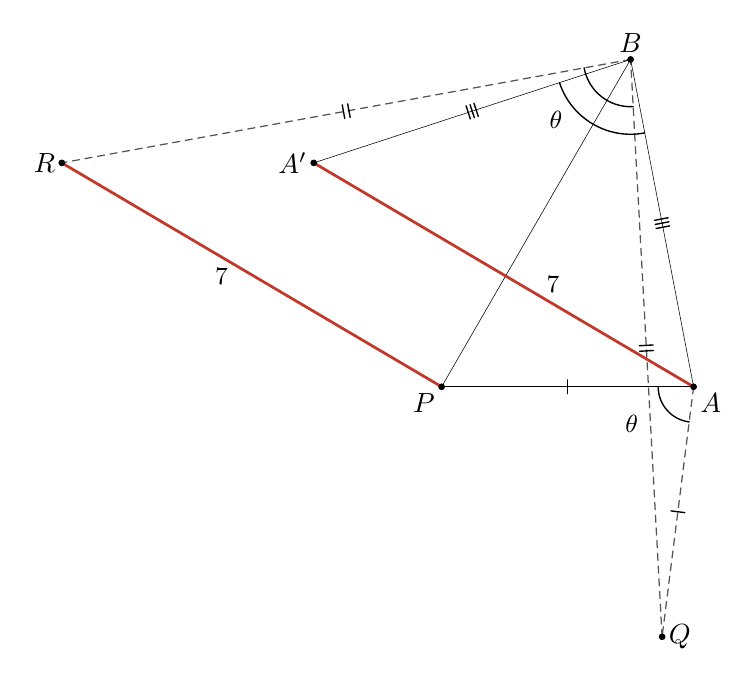
\begin{tikzpicture}
%! let theta = acos(1/8)*180/pi
\tkzDefPoint(0.0,0.0){P} %! P = (0, 0)
\tkzDefPoint(3.2000000,0.0){A} %! A = (4, 0)
\tkzDefPoint(2.4000000,4.1569219){B} %! B = (3, 3*sqrt(3))
\tkzDefPoint(2.8000000,-3.1749016){Q} %! Q = rotate(P, A, theta)
\tkzDefPoint(-4.8243181,2.8435813){R} %! R = rotate(Q, B, -theta)
\tkzDefPoint(-1.6243181,2.8435813){Ap} %! Ap = rotate(A, B, -theta)
%! fact dist(P, A) == 4
%! fact dist(P, B) == 6
%! fact equal(dist(A, B)**2, 28)
%! fact dist(P, R) == 7
%! fact dist(A, Ap) == 7
%! fact parallel(P, R, A, Ap)
%! fact equal(dist(A, Q), dist(A, P))
%! fact equal(dist(B, R), dist(B, Q))
%! fact equal(dist(B, Ap), dist(B, A))
%! fact equal(cosd(angle(P, A, Q)), 1/8)
%! fact equal(cosd(angle(Q, B, R)), 1/8)
\tkzDrawSegments[aux](A,Q Q,B B,R)
\tkzDrawSegments(P,A P,B A,B B,Ap)
\tkzMarkSegments[mark=|,size=2.5pt,mk](P,A A,Q)
\tkzMarkSegments[mark=||,size=2.5pt,mk](Q,B B,R)
\tkzMarkSegments[mark=|||,size=2.5pt,mk](A,B B,Ap)
\tkzDrawSegment[key](P,R)
\tkzDrawSegment[key](A,Ap)
\tkzMarkAngle[size=.45,arc=l,mark=none,mk](P,A,Q)
\tkzMarkAngle[size=.6,arc=l,mark=none,mk](R,B,Q)
\tkzMarkAngle[size=.95,arc=l,mark=none,mk](Ap,B,A)
\tkzDrawPoints(P,A,B,Q,R,Ap)
\tkzLabelSegment[below left,pos=.55,len](P,R){$7$}
\tkzLabelSegment[above right,pos=.4,len](A,Ap){$7$}
\tkzLabelAngle[pos=.72,xshift=-7pt,font=\small](P,A,Q){$\theta$}
\tkzLabelAngle[pos=1.22,font=\small](Ap,B,P){$\theta$}
\tkzLabelPoint[below left,lbl](P){$P$}
\tkzLabelPoint[below right,lbl](A){$A$}
\tkzLabelPoint[above,lbl](B){$B$}
\tkzLabelPoint[right,lbl](Q){$Q$}
\tkzLabelPoint[left,lbl](R){$R$}
\tkzLabelPoint[left,lbl](Ap){$A'$}
\end{tikzpicture}
\end{document}
